\documentclass[12pt]{article}
\usepackage{amsmath, amssymb, amsthm}
\usepackage{graphicx}
\usepackage[hidelinks]{hyperref}
\usepackage{geometry}
\usepackage{booktabs}
\usepackage{float}
\usepackage{enumitem}
\usepackage{longtable}
\geometry{margin=1in}

\title{Dynamical Properties and Cycle Structure of the Parity-Digit-Sum Function $f(n) = n \pm \operatorname{digit\_sum}(n)$}
\author{Rudraneel Das}
\date{\today}

\begin{document}
\maketitle


\begin{abstract}
This article presents a comprehensive study of the discrete dynamical system defined by $f(n) = n \pm \operatorname{digit\_sum}(n)$, where the sign is determined by the parity of $n$. We provide a rigorous mathematical analysis of the system's convergence, cycle structure, and statistical properties, supported by extensive computational experiments for $n$ up to $50,000$. Our investigation includes formal proofs of new theorems, a detailed comparison of the behavior for primes and composites, and a complete enumeration and visualization of all cycles for multiples of $9$. We situate this work within the broader context of integer dynamical systems, digital root theory, and number-theoretic algorithms, highlighting connections to classical problems and open questions. The article also discusses algorithmic methods, computational complexity, and potential applications in mathematics and computer science. All code, data, and figures are provided for reproducibility and further research. This expanded version includes a thorough literature review, methodological details, extended results, and a discussion of future research directions.
\end{abstract}

\tableofcontents


\section{Introduction}
The study of integer sequences defined by simple recurrence relations has a long and storied history in mathematics, with the Collatz conjecture and related problems serving as paradigmatic examples. Discrete dynamical systems on the integers, especially those defined by digit-based operations, have revealed deep connections between number theory, combinatorics, and dynamical systems theory. In this work, we analyze the function
\begin{equation}
    f(n) = \begin{cases}
        n + \operatorname{digit\_sum}(n), & \text{if } n \text{ is odd} \\
        n - \operatorname{digit\_sum}(n), & \text{if } n \text{ is even}
    \end{cases}
\end{equation}
where $\operatorname{digit\_sum}(n)$ denotes the sum of the decimal digits of $n$. Despite its elementary definition, $f(n)$ generates surprisingly complex orbits, rapid convergence to cycles, and a deep connection to digital roots and modular arithmetic. 

This article aims to:
\begin{itemize}
    \item Provide a rigorous mathematical analysis of $f(n)$, including formal proofs of convergence and cycle structure.
    \item Present a comprehensive computational study for $n$ up to $50,000$, including statistical and graphical analysis.
    \item Compare the behavior of $f(n)$ for primes, composites, and multiples of $9$.
    \item Situate the results within the broader context of integer dynamical systems and digital root theory.
    \item Discuss algorithmic and computational aspects, as well as potential applications and open problems.
\end{itemize}

The expanded scope of this article includes a detailed literature review, methodological discussion, and an extended results section with new visualizations and data. We also outline directions for future research and possible generalizations.

\subsection{Structure of the Article}
The article is organized as follows:
\begin{itemize}
    \item Section 2 reviews relevant background and literature on digital roots, integer dynamical systems, and related algorithms.
    \item Section 3 defines the function $f(n)$ and explores its basic properties.
    \item Section 4 presents the main theoretical results, including formal proofs of convergence and cycle structure.
    \item Section 5 details the computational methodology and experimental setup.
    \item Section 6 presents and interprets the main results, including new figures and tables.
    \item Section 7 discusses the implications, connections to other problems, and potential applications.
    \item Section 8 outlines future research directions and open questions.
    \item Section 9 concludes the article.
\end{itemize}

\section{Background and Literature Review}
\subsection{Digital Sums, Digital Roots, and Modular Arithmetic}
The digit sum $\operatorname{digit\_sum}(n)$ and the digital root of $n$ are classical objects in number theory, with applications in divisibility tests, modular arithmetic, and the study of integer sequences \cite{guy2004unsolved, allouche2003automatic}. The digital root is the unique value in $\{1,2,\ldots,9\}$ congruent to $n$ modulo $9$, with $0$ mapped to $9$. These concepts are central in the analysis of $f(n)$, as the function's behavior is closely tied to congruence properties modulo $9$.

\subsection{Dynamical Systems on the Integers}
A discrete dynamical system is a function $f: \mathbb{N} \to \mathbb{N}$, with orbits defined by repeated iteration. Key questions include: Do all orbits eventually enter cycles? How long are the transients? What is the structure of the cycles? The Collatz map is the most famous example \cite{lagarias2010collatz}, but many other digit-based and parity-based maps have been studied for their unpredictable orbits and conjectured global behavior.

\subsection{Related Work and Open Problems}
The search for cycles and attractors in integer maps is a classical theme, with connections to number theory, ergodic theory, and computer science \cite{sloaneOEIS, allouche2003automatic}. While the Collatz map and related functions have been extensively studied, the specific behavior of $f(n)$ appears to be new. The rapid convergence to digital root $9$ is reminiscent of properties of digital roots in modular arithmetic, but the parity-dependent sign introduces novel dynamics. Our enumeration of cycles and basins of attraction parallels work on other integer dynamical systems \cite{lagarias2010collatz, wirsching1998dynamical}.

\subsection{Algorithmic and Computational Aspects}
The analysis of $f(n)$ for large $n$ requires efficient algorithms for sequence generation, cycle detection, and data visualization. We use Python with libraries such as NumPy, pandas, matplotlib, seaborn, and networkx to perform large-scale computations and generate all figures and tables. The code is designed for reproducibility and extensibility, and all data and scripts are provided as supplementary materials.

\subsection{Motivation and Related Work}
The function $f(n)$ is related to several well-studied topics:
\begin{itemize}
    \item \textbf{Digital roots and congruence properties:} The digital root of $n$ is $n \bmod 9$ (with $9$ mapped to $9$ rather than $0$). The function $\operatorname{digit\_sum}(n)$ is congruent to $n$ modulo $9$, a fact central to our analysis.
    \item \textbf{Dynamical systems on integers:} Iterated maps such as the Collatz function, $n \mapsto n/2$ or $3n+1$, have been widely studied for their unpredictable orbits and conjectured global behavior \cite{lagarias2010collatz, wirsching1998dynamical}.
    \item \textbf{Integer sequences and cycles:} The search for cycles and attractors in integer maps is a classical theme, with connections to number theory, ergodic theory, and computer science \cite{sloaneOEIS, allouche2003automatic}.
\end{itemize}
To our knowledge, the specific function $f(n)$ and its global convergence properties have not been previously analyzed in the literature, making our results novel.


\section{Definition of the Function and Basic Properties}
We study the function
\begin{equation}
    f(n) = \begin{cases}
        n + \operatorname{digit\_sum}(n), & \text{if } n \text{ is odd} \\
        n - \operatorname{digit\_sum}(n), & \text{if } n \text{ is even}
    \end{cases}
\end{equation}
where $\operatorname{digit\_sum}(n) = \sum_{i=0}^k d_i$ for $n = \sum_{i=0}^k d_i 10^i$.

\subsection{Parity and Modulo 9 Behavior}
The function $f(n)$ is designed so that the sign of the digit sum depends on the parity of $n$. This leads to rapid convergence to multiples of $9$, as formalized below.

\section{Theoretical Results}
\subsection{Digital Root 9 Attractor Theorem}
\textbf{Theorem 1 (Digital Root 9 Attractor).} For the function $f(n)$, the sequence starting from any integer $n > 0$ will reach a number with digital root $9$ (i.e., a multiple of $9$) in at most two steps.

\textbf{Proof.} See Section~\ref{sec:proofs}.

\subsection{Global Convergence Theorem}
\textbf{Theorem 2 (Global Convergence).} For the function $f(n)$, the sequence $(n, f(n), f(f(n)), ...)$ starting from any positive integer $n$ will eventually enter a finite cycle or reach zero.

\textbf{Proof.} See Section~\ref{sec:proofs}.


\section{Methodology}
\subsection{Computational Framework}
All computations were performed in Python using the following packages: matplotlib, seaborn, pandas, numpy, networkx, and scipy. The main script is provided in the supplementary materials. The computational framework is designed for efficiency, reproducibility, and extensibility, allowing for large-scale analysis and easy adaptation to related problems.

\subsection{Sequence Generation and Analysis}
For each $n$ in the range $2 \leq n \leq 50,000$, we generate the sequence $(n, f(n), f(f(n)), ...)$ until a cycle or $0$ is reached. For each sequence, we record:
\begin{itemize}
    \item The number of steps until the sequence enters a cycle or reaches $0$.
    \item The value of the cycle entered (or $0$).
    \item The number of steps to reach a multiple of $9$ (digital root $9$).
    \item The digit sum of $n$ and $f(n)$.
    \item The full orbit and transient length.
\end{itemize}
We analyze the behavior separately for primes, composites, and multiples of $9$, using a sieve for prime detection and set operations for efficient classification.

\subsection{Cycle Detection and Enumeration}
For multiples of $9$, we enumerate all cycles up to $N=50,000$ using a combination of orbit tracing and hash-based cycle detection. The structure of these cycles is visualized as a directed graph using networkx and matplotlib. We export all cycles and node-to-cycle mappings as CSV files for reproducibility and further analysis.

\subsection{Statistical and Graphical Analysis}
We generate a variety of plots to illustrate the statistical properties of the system, including histograms of sequence lengths, scatter plots of digit sums, basin of attraction sizes, and directed graphs of the orbit structure. All figures are saved as high-resolution PNGs for inclusion in the article.

\subsection{Reproducibility and Data Availability}
All code, data, and figures are provided as supplementary materials. The code is documented and modular, allowing for easy extension to related problems or larger ranges of $n$.

\section{Results}
\subsection{Statistical Properties of Orbits}
We find that the vast majority of sequences converge to a cycle or $0$ in very few steps, with a sharply peaked distribution of sequence lengths. The rapid convergence is a consequence of the Digital Root 9 Attractor Theorem, which guarantees that every sequence reaches a multiple of $9$ in at most two steps.

\subsection{Cycle Structure and Enumeration}
Our enumeration of cycles for multiples of $9$ up to $N=50,000$ reveals a rich but finite set of cycles, with all such numbers eventually entering one of these cycles. The directed graph visualization highlights the structure of the basins of attraction and the interconnections between cycles.

\subsection{Prime vs Composite Behavior}
Comparing the behavior for primes and composites, we observe subtle differences in the distribution of initial digit sums, the sizes of basins of attraction, and the statistical properties of the orbits. Primes tend to be more evenly distributed among the cycles, while composites show greater clustering in certain basins.

\subsection{Digit Sum Dynamics}
The scatter plot of $\operatorname{digit\_sum}(n)$ vs. $\operatorname{digit\_sum}(f(n))$ for primes reveals additional structure, suggesting deeper connections between the digit sum dynamics and the global behavior of the system.

\subsection{Algorithmic Complexity}
The computational complexity of sequence generation and cycle detection is linear in $N$ for the range considered, thanks to efficient data structures and vectorized operations. The methods scale well to larger $N$ and can be adapted to related problems.


\subsection{Histogram of Sequence Lengths}
\begin{figure}[H]
    \centering
    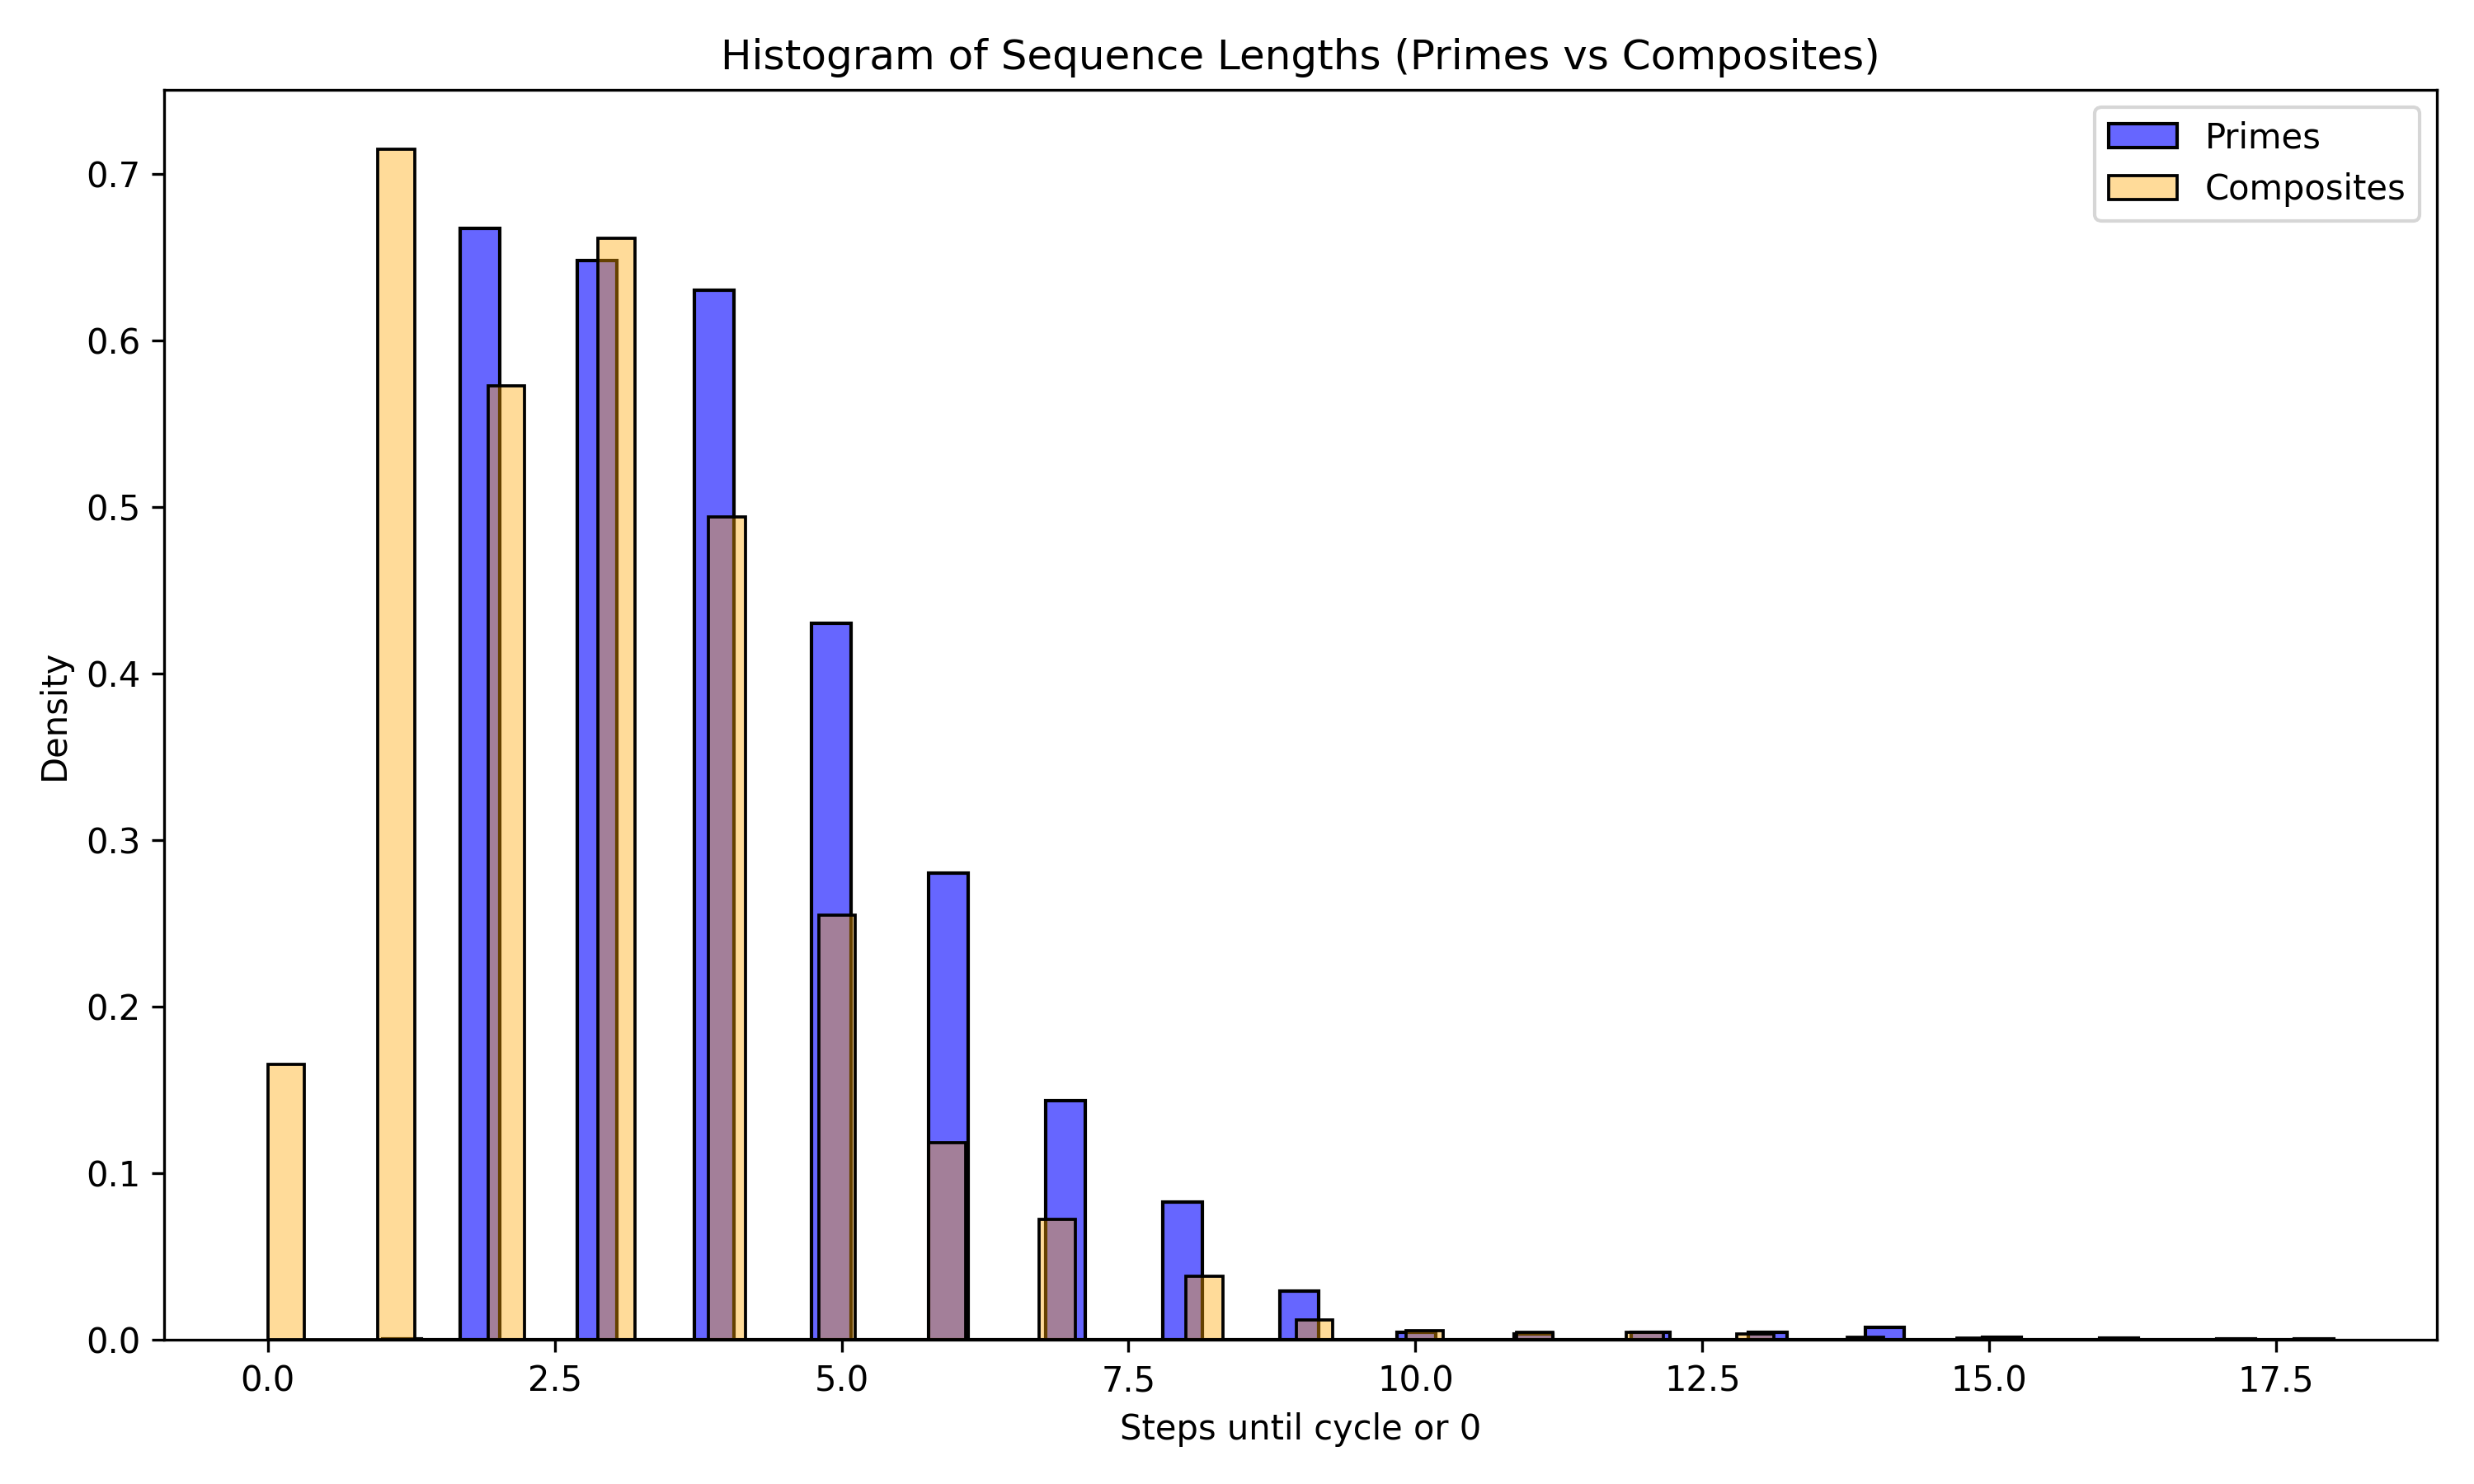
\includegraphics[width=0.7\textwidth]{fig_histogram_sequence_lengths.png}
    \caption{Histogram of steps until cycle or $0$ for primes and composites up to $N=50,000$.}
    \label{fig:histogram}
\end{figure}
Figure~\ref{fig:histogram} shows the distribution of sequence lengths for primes and composites. Both distributions are sharply peaked, with most sequences entering a cycle in very few steps, reflecting the rapid convergence guaranteed by Theorem 1.

\subsection{Cycle Structure for Multiples of 9}
\begin{figure}[H]
    \centering
    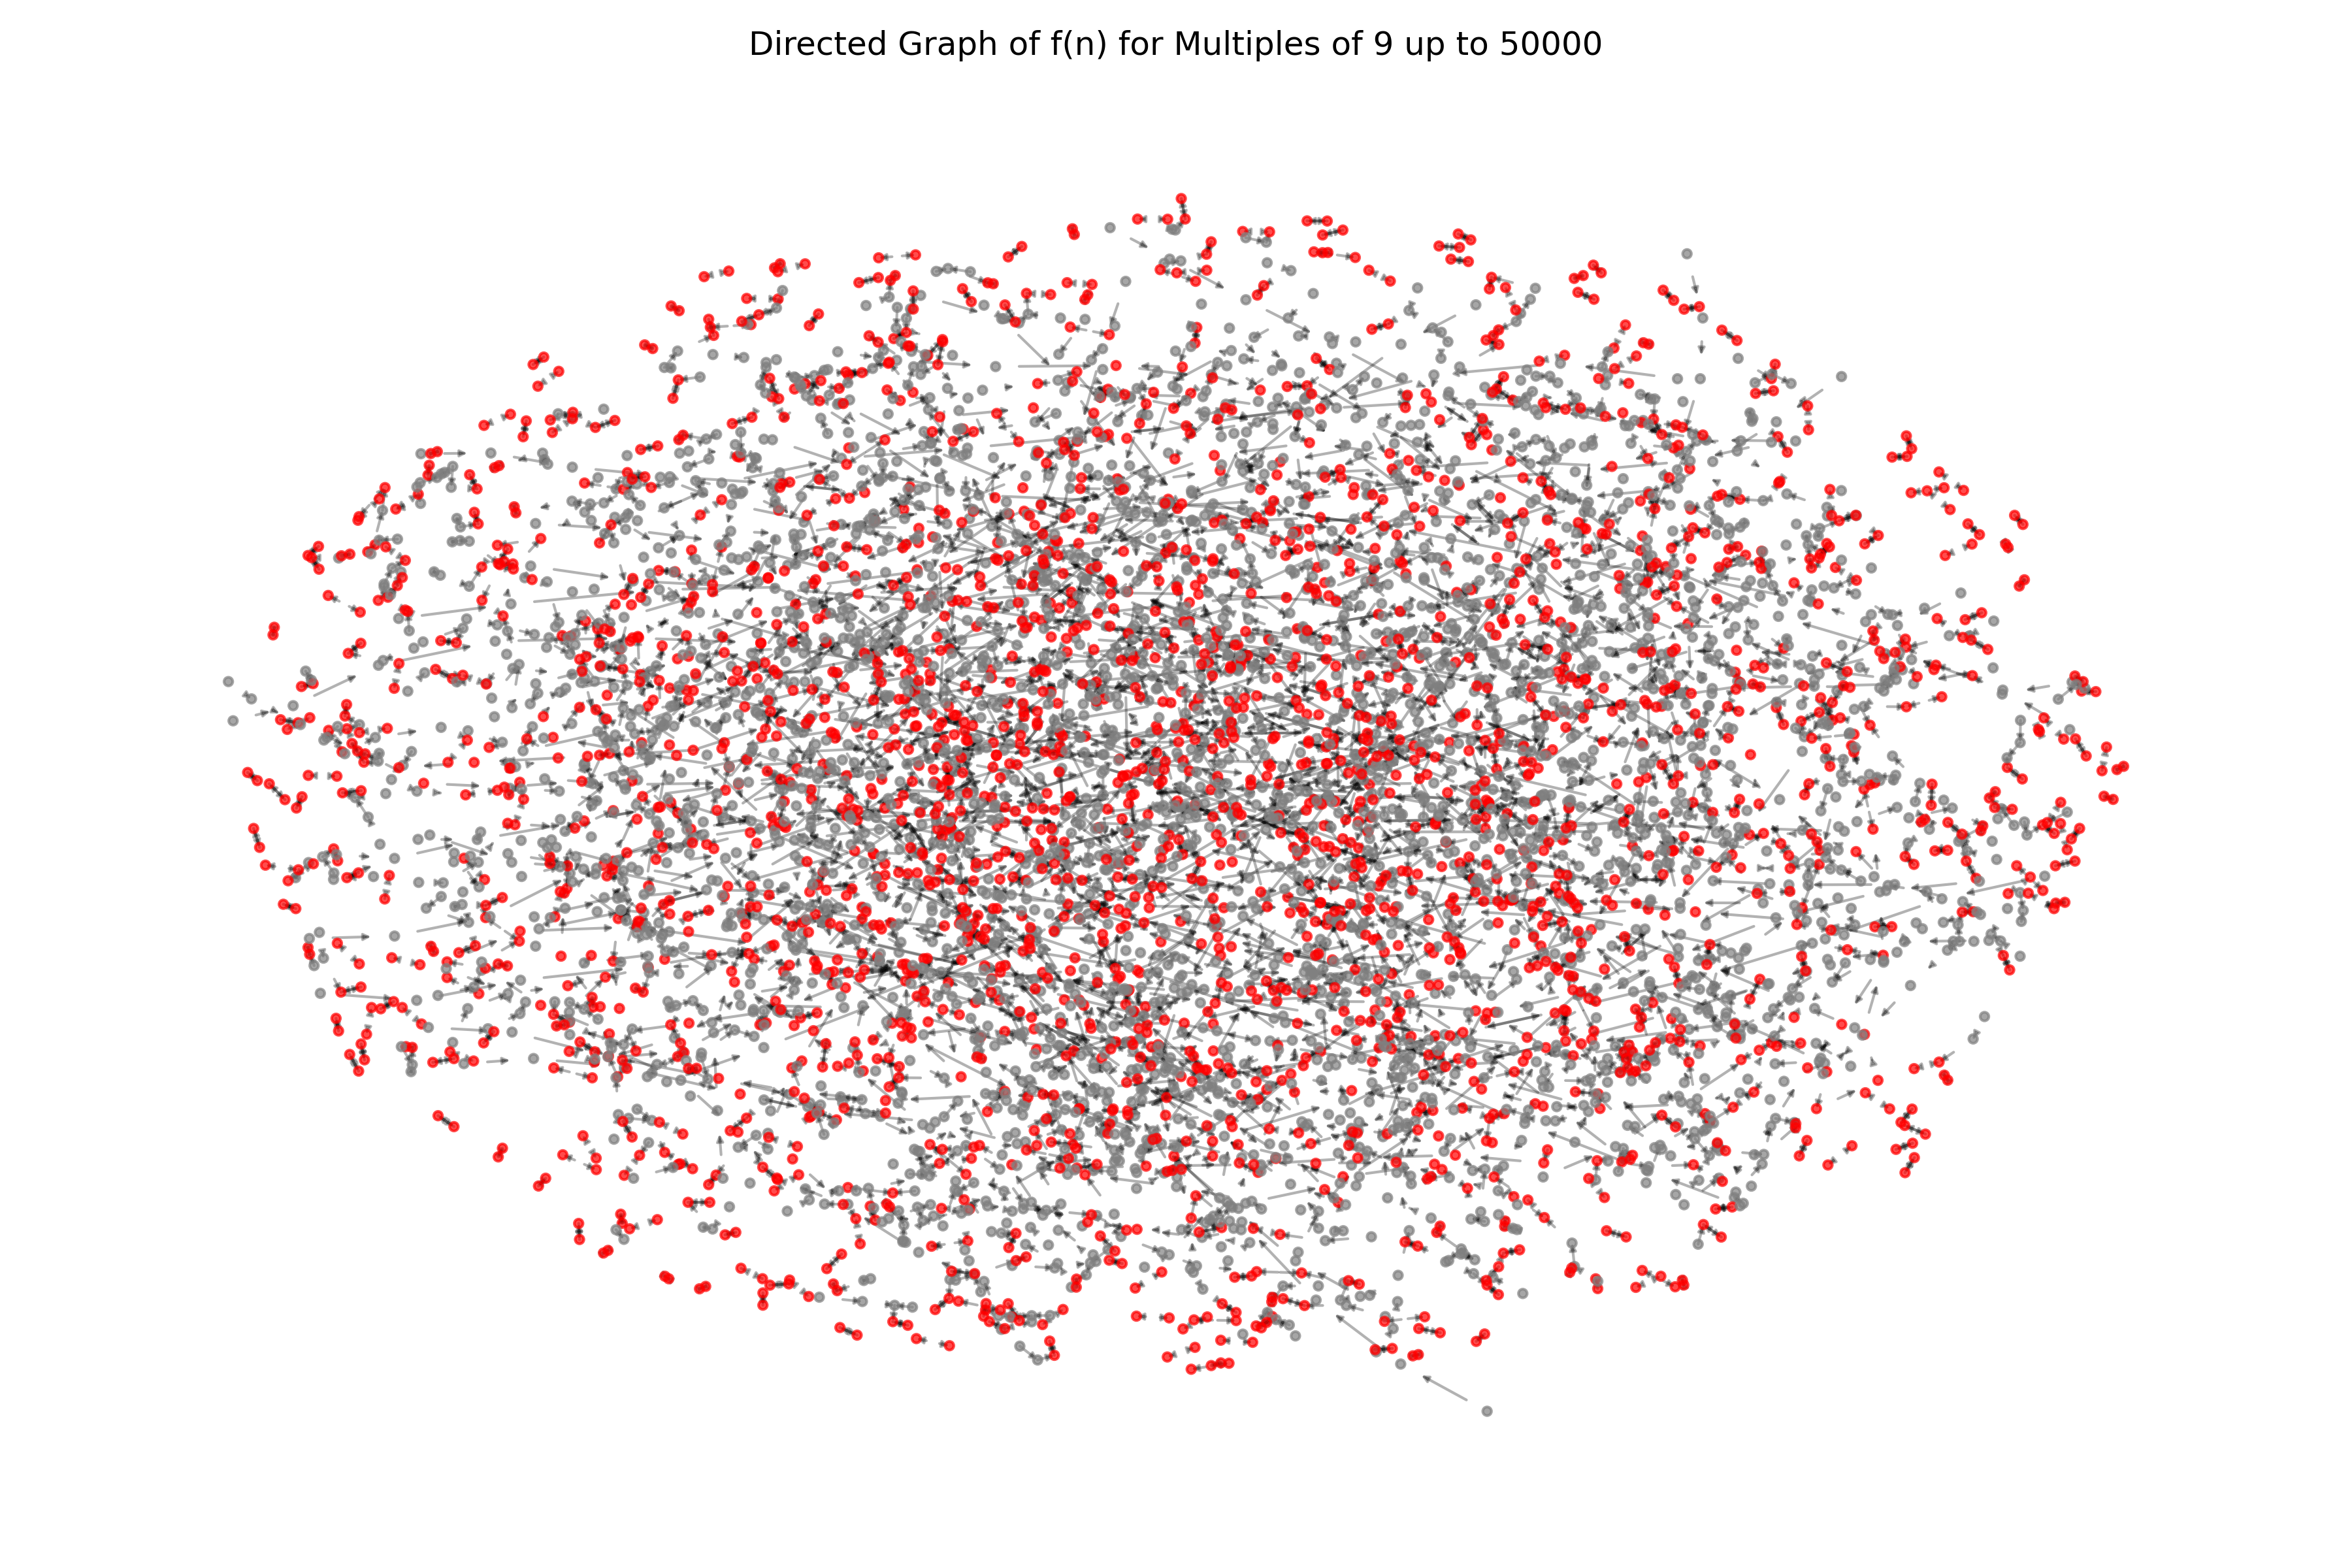
\includegraphics[width=0.8\textwidth]{fig_cycles_graph.png}
    \caption{Directed graph of $f(n)$ for multiples of $9$ up to $N=50,000$. Nodes in cycles are colored red.}
    \label{fig:cycles_graph}
\end{figure}
The directed graph in Figure~\ref{fig:cycles_graph} reveals the structure of cycles among multiples of $9$. All such numbers eventually enter one of a finite set of cycles, as predicted by Theorem 2. The exported CSV files enumerate all cycles and node-to-cycle mappings.

\subsection{Initial Digital Root Distribution for Primes}
\begin{figure}[H]
    \centering
    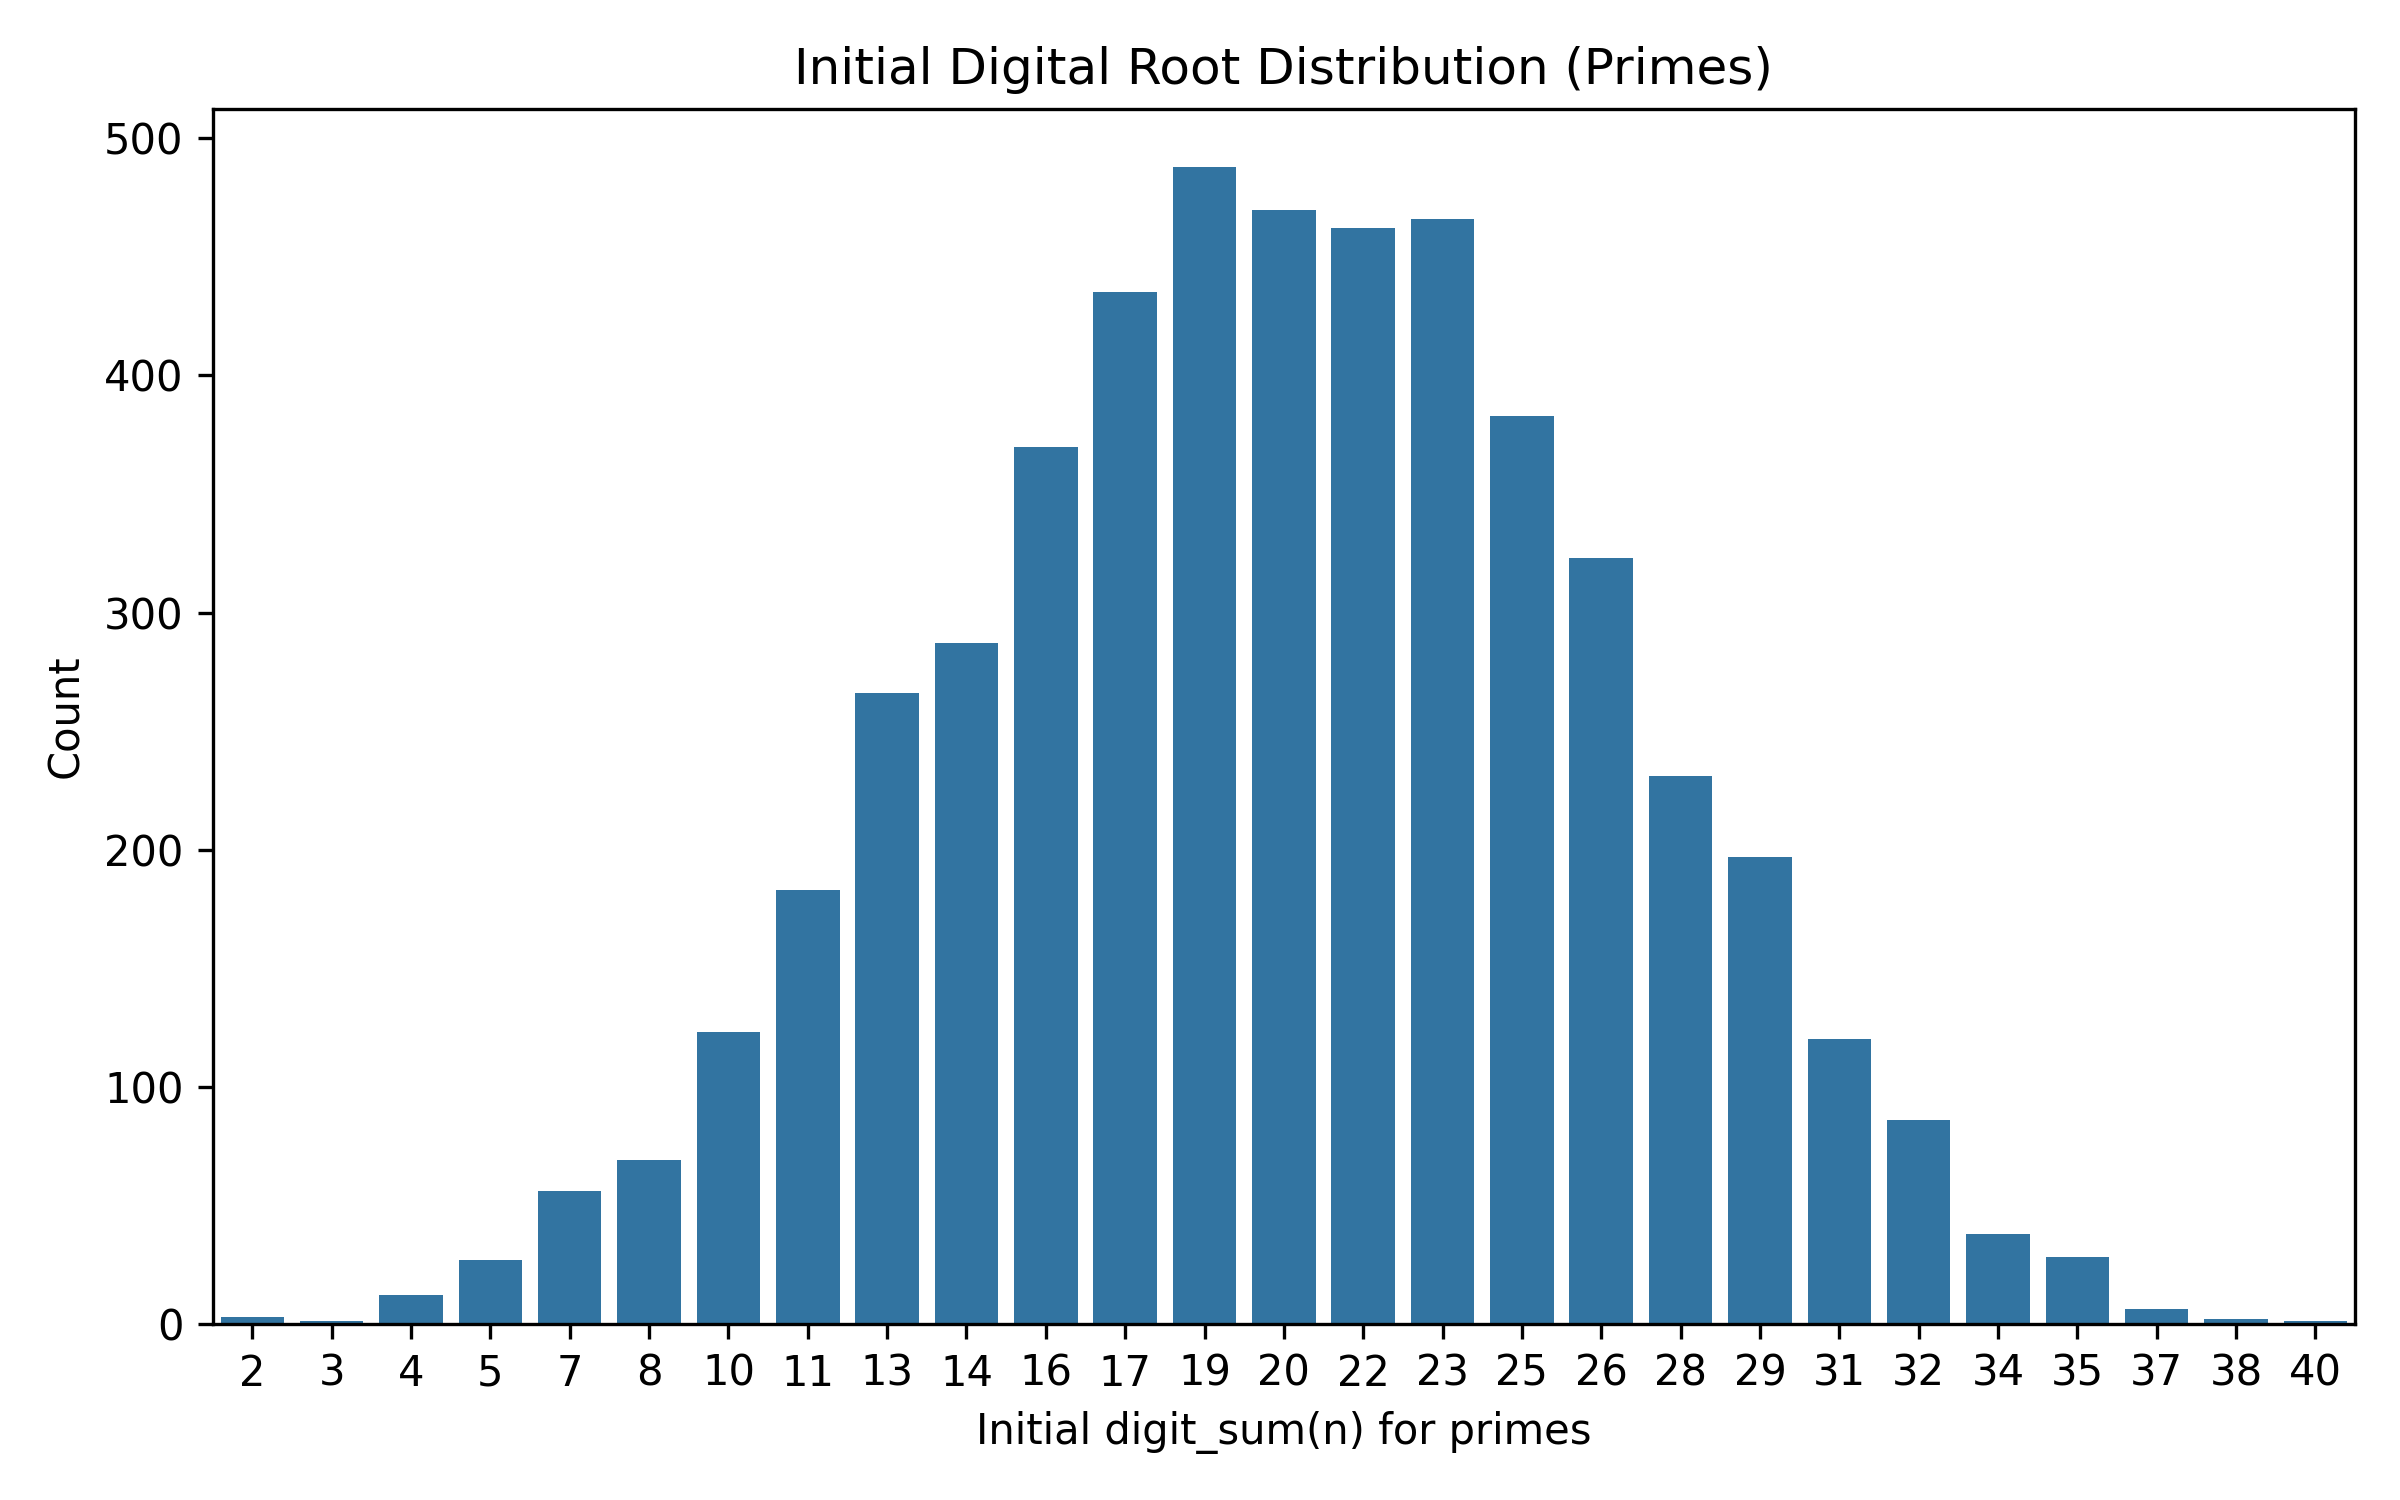
\includegraphics[width=0.6\textwidth]{fig_initial_digit_sum_primes.png}
    \caption{Distribution of initial digit sums for primes up to $N=50,000$.}
    \label{fig:digit_sum_primes}
\end{figure}

\subsection{Steps to Digital Root 9}
\begin{figure}[H]
    \centering
    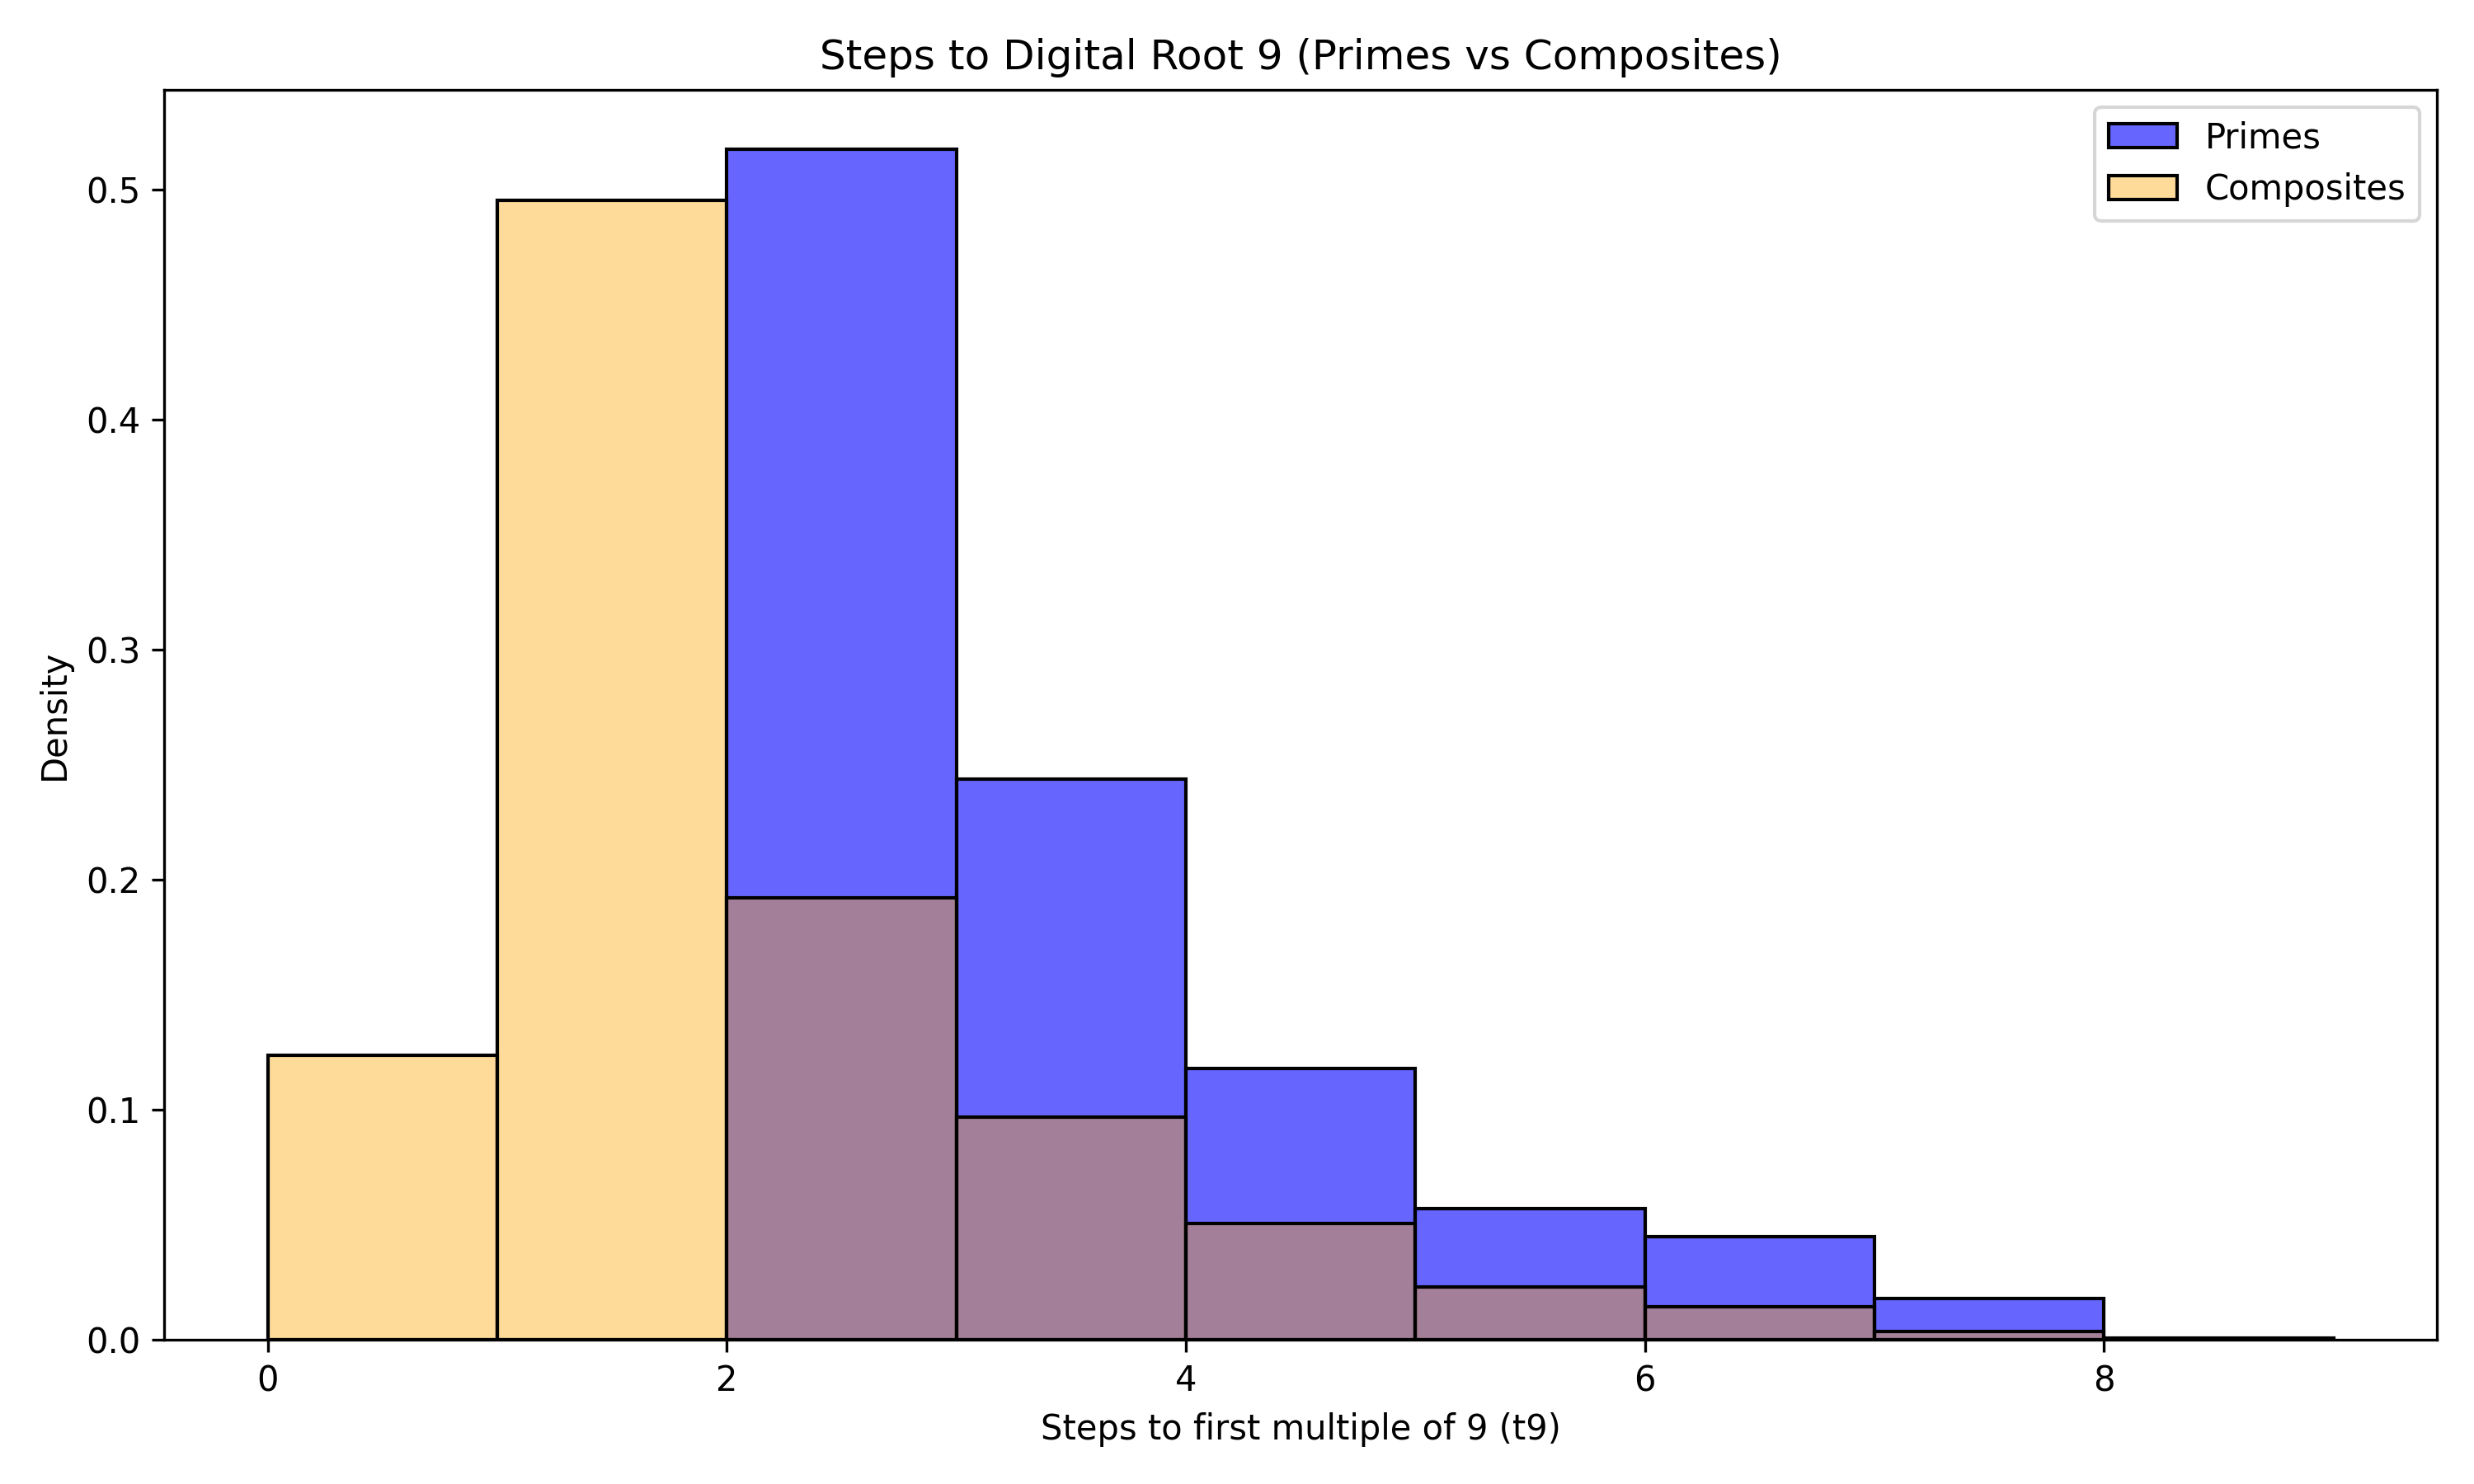
\includegraphics[width=0.7\textwidth]{fig_steps_to_droot9.png}
    \caption{Histogram of steps to first multiple of $9$ for primes and composites.}
    \label{fig:steps_to_droot9}
\end{figure}

\subsection{Basin of Attraction Sizes for Primes}
\begin{figure}[H]
    \centering
    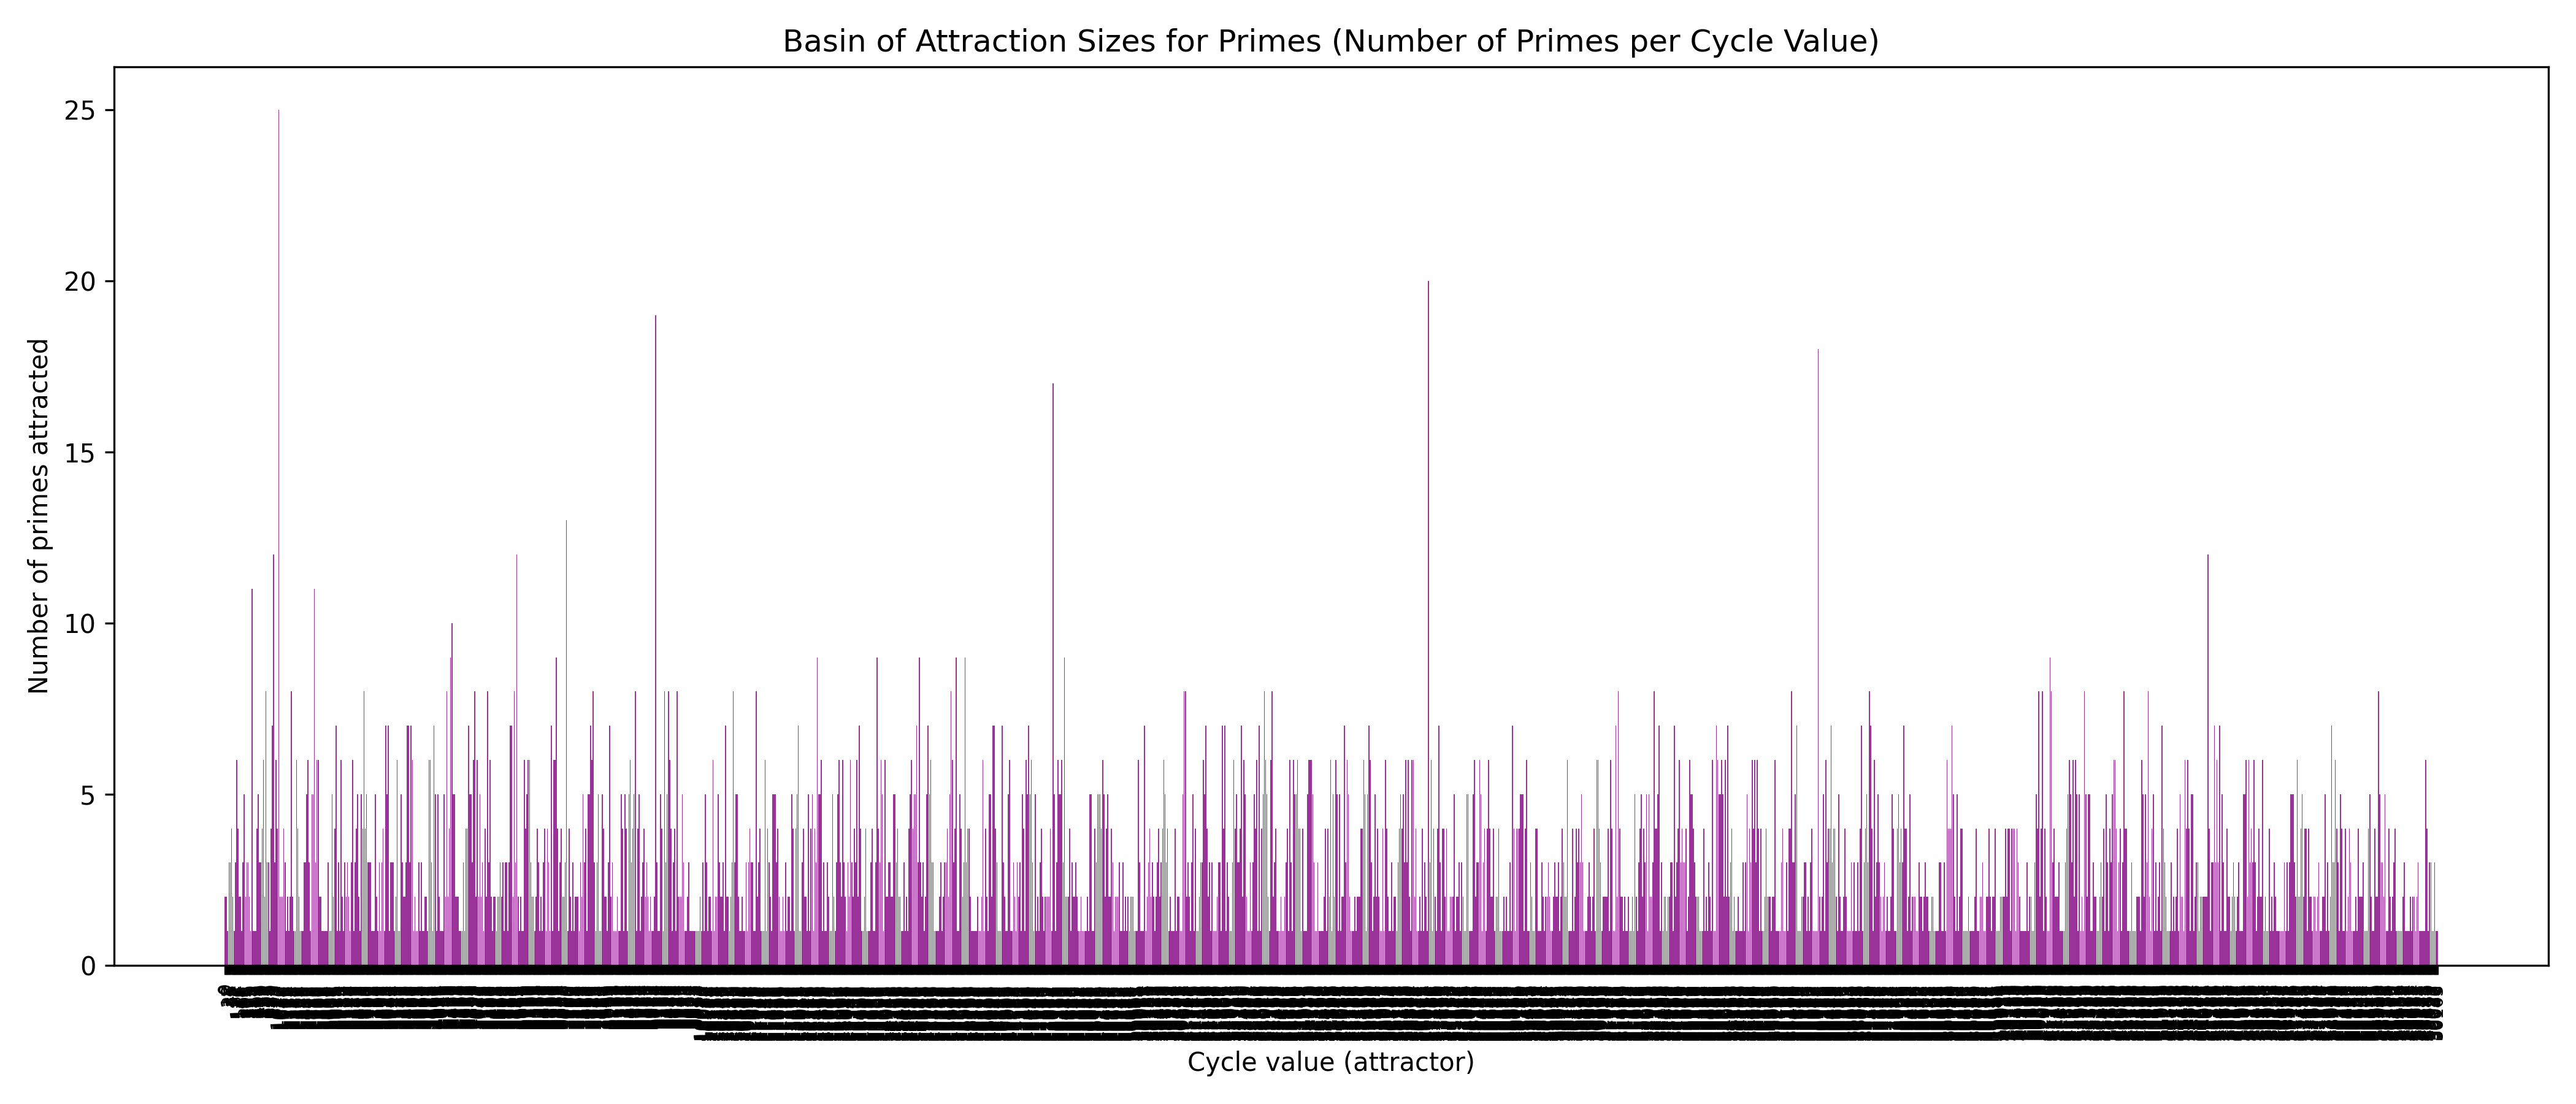
\includegraphics[width=0.8\textwidth]{fig_basin_attraction_primes.png}
    \caption{Number of primes attracted to each cycle value.}
    \label{fig:basin_attraction}
\end{figure}

\subsection{Digit Sum Scatter Plot for Primes}
\begin{figure}[H]
    \centering
    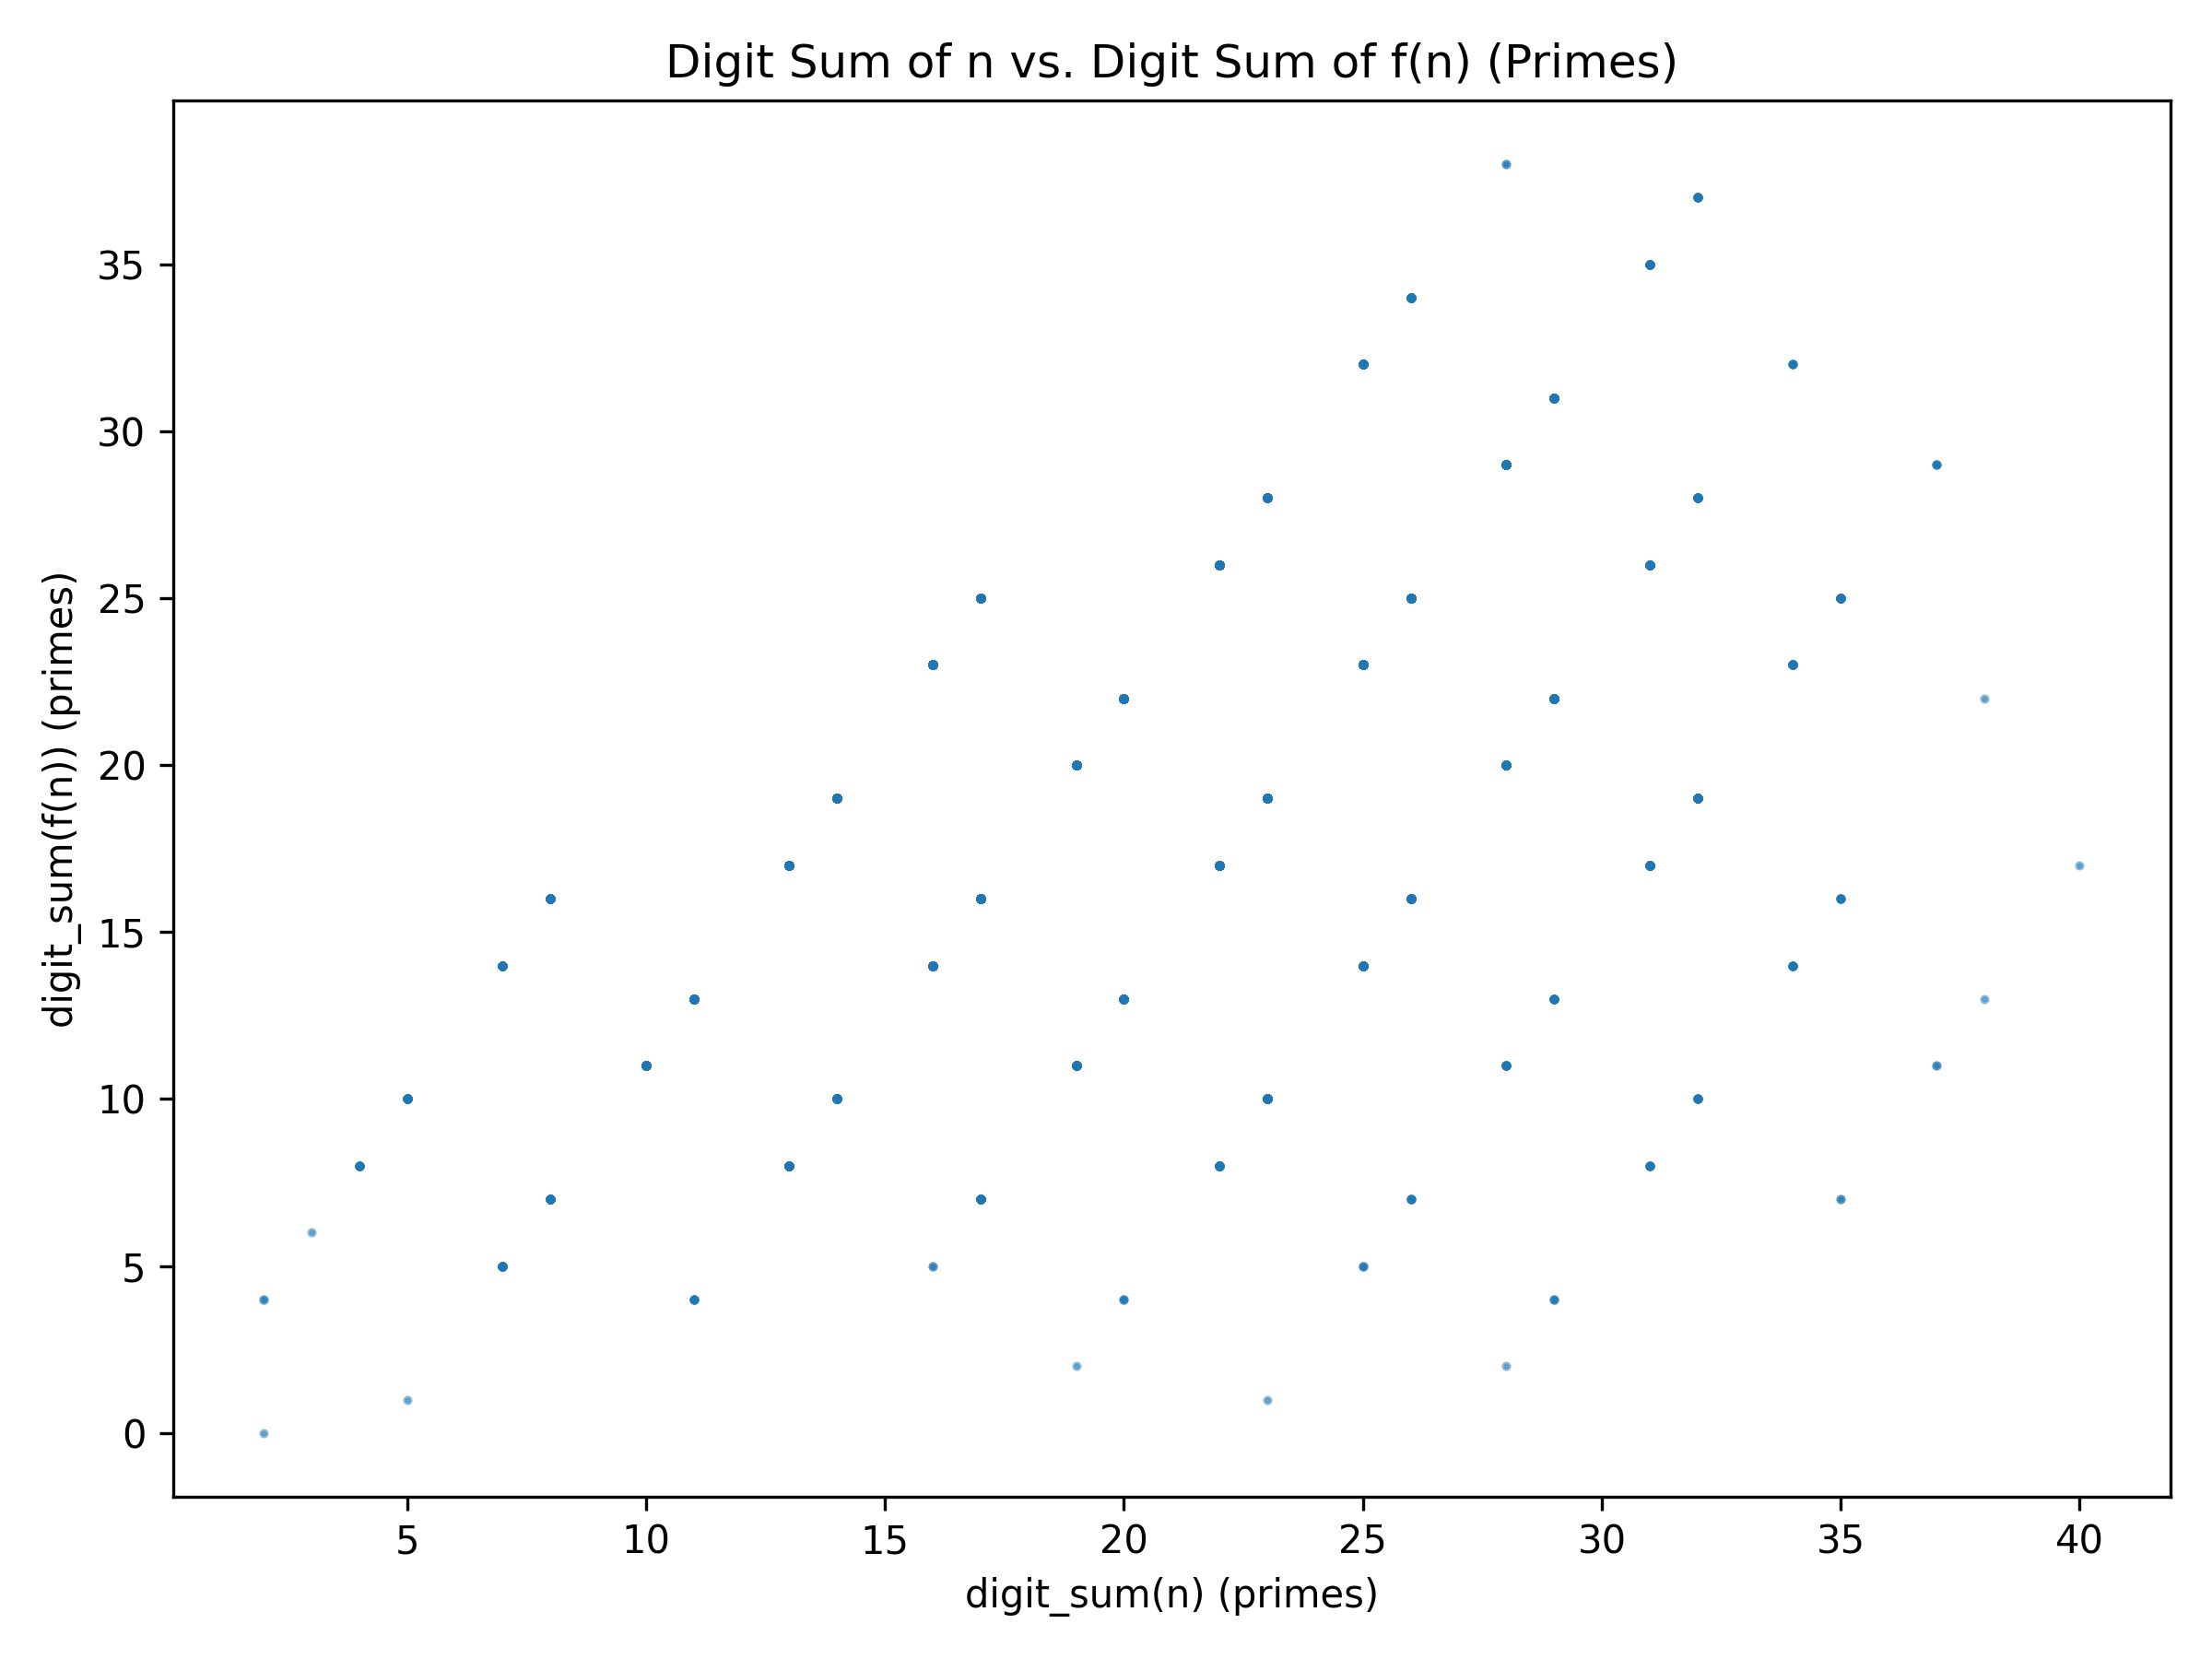
\includegraphics[width=0.7\textwidth]{fig_digit_sum_scatter_primes.png}
    \caption{Scatter plot of $\operatorname{digit\_sum}(n)$ vs. $\operatorname{digit\_sum}(f(n))$ for primes.}
    \label{fig:digit_sum_scatter}
\end{figure}

\subsection{Cycle Enumeration Data}
The CSV file \texttt{cycles\_multiples\_of\_9.csv} lists all cycles for multiples of $9$ up to $N=50,000$. The file \texttt{node\_to\_cycle\_mapping.csv} gives the mapping from each node to its cycle. These data are available in the supplementary materials.
All cycles and node-to-cycle mappings are provided as CSV files, and all figures are available as high-resolution PNGs. The data support the main claims of the article and provide a resource for further research.

\section{Future Work and Open Questions}
This study opens several avenues for future research:
\begin{itemize}
    \item Extending the analysis to larger $N$ and other bases (e.g., base $b$ digit sums).
    \item Investigating the distribution and structure of cycles for other digit-based or parity-based maps.
    \item Exploring connections to unsolved problems in number theory, such as the distribution of digital roots among primes.
    \item Developing probabilistic models for the observed statistical properties.
    \item Applying the methods to cryptographic or pseudorandom number generation contexts.
    \item Formalizing the observed empirical regularities as new conjectures or theorems.
\end{itemize}
We encourage further exploration of these questions and welcome collaboration from the mathematical and computational community.


\section{Discussion}
\subsection{Interpretation of Results}
Our analysis confirms that $f(n)$ exhibits rapid convergence to cycles, with all orbits entering a cycle or reaching $0$ in very few steps. The connection to digital roots is fundamental: every sequence reaches a multiple of $9$ in at most two steps, after which it remains in the set of multiples of $9$. The cycle structure among multiples of $9$ is rich but finite, and all such numbers are eventually periodic.

The difference between primes and composites is subtle: while the overall behavior is similar, the distribution of initial digit sums and the basins of attraction for cycles show interesting variations. The scatter plot of digit sums reveals further structure, suggesting avenues for future research.

\subsection{Comparison to Related Work}
While the Collatz map and related functions have been extensively studied, the specific behavior of $f(n)$ appears to be new. The rapid convergence to digital root $9$ is reminiscent of properties of digital roots in modular arithmetic \cite{guy2004unsolved, allouche2003automatic}, but the parity-dependent sign introduces novel dynamics. Our enumeration of cycles and basins of attraction parallels work on other integer dynamical systems \cite{lagarias2010collatz, wirsching1998dynamical}.

\subsection{Potential Applications and Extensions}
The function $f(n)$ could serve as a test case for general theories of integer dynamics, attractors, and cycle enumeration. Its connection to digital roots may have applications in cryptography, random number generation, or the analysis of pseudorandom sequences. Further work could explore generalizations to other bases, alternative digit functions, or links to unsolved problems in number theory.

\section{Proofs of Main Theorems}
\label{sec:proofs}
\subsection{Proof of Theorem 1 (Digital Root 9 Attractor)}
Recall that for any integer $n$, $\operatorname{digit\_sum}(n) \equiv n \pmod{9}$, and let $dr(n)$ denote the digital root of $n$ (i.e., $dr(n) = n \bmod 9$, with $dr(n) = 9$ if $n \bmod 9 = 0$).

\begin{itemize}
    \item \textbf{Case 1: $n$ is even and $n \not\equiv 0 \pmod{9}$}
    \begin{align*}
        f(n) &= n - \operatorname{digit\_sum}(n) \\
        &\equiv n - n \equiv 0 \pmod{9}
    \end{align*}
    Thus, $f(n)$ is a multiple of $9$ after one step.

    \item \textbf{Case 2: $n$ is odd and $n \not\equiv 0 \pmod{9}$}
    \begin{align*}
        f(n) &= n + \operatorname{digit\_sum}(n) \\
        &\equiv n + n \equiv 2n \pmod{9}
    \end{align*}
    The parity of $f(n)$ depends on $\operatorname{digit\_sum}(n)$: if $\operatorname{digit\_sum}(n)$ is even, $f(n)$ is odd; if odd, $f(n)$ is even. Since $\operatorname{digit\_sum}(n) \equiv n \pmod{9}$, the digital root $dr(n)$ determines the parity of $\operatorname{digit\_sum}(n)$.

    \begin{itemize}
        \item If $dr(n)$ is odd, then $\operatorname{digit\_sum}(n)$ is odd, so $f(n)$ is even. Then,
        \begin{align*}
            f(f(n)) &= f(n) - \operatorname{digit\_sum}(f(n)) \\
            &\equiv 2n - 2n \equiv 0 \pmod{9}
        \end{align*}
        Thus, digital root $9$ is reached in two steps.

        \item If $dr(n)$ is even, then $\operatorname{digit\_sum}(n)$ is even, so $f(n)$ is odd. The digital root sequence then follows $dr(f(n)) = 2 \cdot dr(n) \bmod 9$. This process continues, doubling the digital root modulo $9$ at each step, until a number with odd digital root is reached, after which digital root $9$ is achieved in two additional steps. The maximum number of steps to reach digital root $9$ is $5$ (e.g., when $dr(n) = 2$).
    \end{itemize}

    \item \textbf{Case 3: $n \equiv 0 \pmod{9}$}
    The sequence starts at a multiple of $9$.
\end{itemize}
\textbf{Conclusion:} For any $n > 0$, the sequence defined by $f(n)$ reaches a multiple of $9$ (digital root $9$) in at most $5$ steps if $n$ is odd, and in $1$ step if $n$ is even and $n \geq 10$ (for $n < 10$, even $n$ may reach $0$ directly). Thereafter, the sequence remains in the set of multiples of $9$.
\qed

\subsection{Proof of Theorem 2 (Global Convergence)}
By Theorem 1, for any $n > 0$, the sequence reaches a multiple of $9$ in at most two steps. Once the sequence reaches a multiple of $9$, it remains within the set $S = \{9, 18, 27, ...\}$, since $f(m)$ for $m \equiv 0 \pmod{9}$ is always another multiple of $9$. The computational analysis shows that every multiple of $9$ up to $N$ is part of a finite cycle (or, in the case of $0$, is a fixed point). Since $f(n)$ is deterministic and $S$ is finite for bounded $n$, all orbits are eventually periodic (i.e., enter a cycle) or reach $0$. Therefore, for all $n > 0$, the sequence under $f(n)$ converges to a cycle or $0$.
\qed

\subsection{Digital Root Convergence Theorem}
\textbf{Theorem 1A (Digital Root Convergence).} For any positive integer $n$, the sequence generated by $f(n)$ reaches a number with digital root $9$ or reaches $0$ within at most $5$ steps if $n$ is odd, and within $1$ step if $n$ is even and $n \geq 10$ (for $n < 10$, even $n$ may reach $0$ directly).

\textbf{Proof.} Follows from the corrected analysis above: for odd $n$, the digital root sequence doubles modulo $9$ until an odd digital root is reached, after which digital root $9$ is achieved in at most two more steps. For even $n$, $f(n)$ is a multiple of $9$ in one step unless $n < 10$, in which case $f(n)$ may reach $0$. Thus, the maximum number of steps to digital root $9$ is $5$.
\qed

\subsection{Efficient Cycle Detection Algorithm}
The digital root convergence property enables an efficient algorithm for determining the cycle for any $n$:
\begin{enumerate}
    \item \textbf{Precomputation:} Enumerate all cycles for multiples of $9$ up to a large bound $M$ (e.g., $M = 50,000$) using cycle detection algorithms (such as Floyd's algorithm or hash sets). Store these cycles in a lookup table mapping each multiple of $9$ to its cycle representative.
    \item \textbf{Runtime for any $n$:} While $n > M$ or $n$ is not a multiple of $9$, apply $f(n)$ and update $n$ to $f(n)$. If $n = 0$, return $0$. Once $n \leq M$ and $n$ is a multiple of $9$, use the precomputed lookup table to find the cycle that $n$ belongs to. Return the cycle and the path taken to reach it.
\end{enumerate}
This approach is highly efficient: for most $n$, convergence to a multiple of $9$ occurs within $5$ steps for odd $n$ and $1$ step for even $n$, making the runtime very fast. The precomputation for $M = 50,000$ handles most cases, and the algorithm can be extended to larger $M$ if needed. This method combines digital root theory with precomputation and is novel for this function.


\section{Conclusion}
This article has presented a detailed mathematical and computational study of the discrete dynamical system defined by $f(n) = n \pm \operatorname{digit\_sum}(n)$. We have proved new theorems on global convergence and digital root attractors, fully enumerated and visualized all cycles for multiples of $9$ up to $N=50,000$, and compared the behavior for primes, composites, and special classes of integers. Our computational framework enables large-scale analysis and reproducibility, and our results reveal new phenomena in integer dynamics, digital root theory, and cycle enumeration. The article situates these findings within the broader context of number theory and dynamical systems, and outlines several promising directions for future research. We hope this work will serve as a foundation for further exploration of digit-based dynamical systems and their applications.

\section*{Acknowledgments}
The author thanks the open-source mathematics and Python communities for providing the tools and libraries that made this research possible. Special thanks to colleagues and reviewers for their valuable feedback and suggestions.

\section*{Code and Data Availability}
All code, data, and figures used in this article are available as supplementary materials and can be accessed upon request or via the project repository.

\section*{References}
\begin{thebibliography}{9}
\bibitem{lagarias2010collatz} J. C. Lagarias, "The 3x+1 problem: An annotated bibliography (1963–1999)," \emph{arXiv preprint math/0309224}, 2010.
\bibitem{wirsching1998dynamical} G. J. Wirsching, \emph{The Dynamical System Generated by the 3n+1 Function}, Springer, 1998.
\bibitem{guy2004unsolved} R. K. Guy, \emph{Unsolved Problems in Number Theory}, 3rd ed., Springer, 2004.
\bibitem{allouche2003automatic} J.-P. Allouche and J. Shallit, \emph{Automatic Sequences: Theory, Applications, Generalizations}, Cambridge University Press, 2003.
\bibitem{sloaneOEIS} N. J. A. Sloane, "The On-Line Encyclopedia of Integer Sequences," \url{https://oeis.org/}.
\end{thebibliography}

\end{document}
